\documentclass[12pt,a4paper]{amsart}
\usepackage{amsfonts}
\usepackage{amsthm}
\usepackage{amsmath}
\usepackage{amscd}
\usepackage[latin2]{inputenc}
\usepackage{t1enc}
\usepackage[mathscr]{eucal}
\usepackage{indentfirst}
\usepackage{graphicx}
\usepackage{graphics}
\usepackage{pict2e}
\usepackage{epic}
\numberwithin{equation}{section}
\usepackage[margin=2.9cm]{geometry}
\usepackage{epstopdf}
\usepackage{bbm}
\usepackage{amsmath,amsfonts,amssymb}
\usepackage{relsize}
\usepackage{mathtools}
\usepackage{commath}
\usepackage{listings}
\usepackage{tabu}
\usepackage{verbatim}
\usepackage{url}
\usepackage{graphicx}
\graphicspath{ {./} }
\usepackage{float}
\usepackage[rightcaption]{sidecap}
 \def\numset#1{{\\mathbb #1}}

 

\theoremstyle{plain}
\newtheorem{Th}{Theorem}[section]
\newtheorem{Lemma}[Th]{Lemma}
\newtheorem{Cor}[Th]{Corollary}
\newtheorem{Prop}[Th]{Proposition}

 \theoremstyle{definition}
\newtheorem{Def}[Th]{Definition}
\newtheorem{Conj}[Th]{Conjecture}
\newtheorem{Rem}[Th]{Remark}
\newtheorem{?}[Th]{Problem}
\newtheorem{Ex}[Th]{Example}

\newcommand{\im}{\operatorname{im}}
\newcommand{\Hom}{{\rm{Hom}}}
\newcommand{\diam}{{\rm{diam}}}
\newcommand{\ovl}{\overline}
% questi sono quelli che ho impostato io
\newcommand{\tr}{^{\mathsmaller T}}
\newcommand{\ones}{\mathbbm{1}}

\begin{document}

\title{P.E.R. nel calcolo del Pagerank:   un confronto sulla scelta del precondizionatore}


\author{Lorenzo Beretta}

\maketitle

\section{Introduzione} Il problema del PageRank risulta essere equivalente alla risoluzione del sistema lineare indotto da una $M$-matrice stocastica.\\
Nell'articolo \cite{Tudisco} gli autori espongono una generalizzazione dei metodi delle potenze e di Jacobi per risolvere tali sistemi che prevede lo splitting di tale matrice indotto dalla proiezione su un'algebra di matrici.\\
Ne propongono poi una nuova particolarizzazione, il metodo HPER (\textit{Householder preconditioned Euler-Richardson}), ottenuta proiettando rispetto all'algebra $sdH$ delle matrici simultaneamente diagonalizzate da un'opportuna matrice di Householder $H$. \\ In quanto segue esporr\'o brevemente il metodo e fornir\'o un'analisi della complessit\'a ed uno studio sperimentale dell'efficienza.

\section{Riduzione ad un sistema lineare}

Sia $G$ la matrice di adiacenza del grafo diretto del web, e sia $A\tr$ la matrice ottenuta da $G$ sostituendo le righe nulle (in corrispondenza dei \textit{dangling nodes}) con $\ones\tr$  e rinormalizzando ogni riga in modo che $A$ risulti stocastica.\\
Allora il problema del pagerank, dati il vettore di personalizzazione $v$ tale che $v\tr\ones=1$ ed il paramentro $\tau \in \left(0,1\right)$ diviene
\begin{equation}
(\tau A + (1-\tau) v \ones\tr)p=p \iff (I-\tau A)p=(1-\tau)v.
\label{sistema}
\end{equation}
Che equivale ad $Mp=y$ per la $M$-matrice stocastica  $M=I-\tau A$ e per $y=(1-\tau)v$, in quanto segue ci occuperemo della risoluzione di questa classe di sistemi.
%In (****citazione****) viene mostrato che pi\'u in generale %esiste una bigezione tra i sistemi lineari di $M$-$matrici$ %%$stoacastiche$ e i problemi di trovare la distribuizone %ergodica di una matrice stocastica che ne defisce %l'equivalenza. [.....posso aggiungere quanto trovato %sull'articolo......]

\section{Il metodo di Euler-Richardson precondizionato}

Il metodo PER (\textit{preconditioned Euler-Richardson}) per la risoluzione del sistema $Mx=y$ consiste nella scelta di un precondizionatore non singolare $P$ che attraverso lo splitting $M=P-(P-M)$ ci fornisce il seguente schema iterativo:
\begin{equation}
x_{k+1}=P^{-1}y+(I-P^{-1}M)x_k 
\end{equation}
Lo stesso metodo delle potenze pu\'o essere interpretato come un PER con la scelta del precondizionatore $P_{PM}=I-\frac{\tau}{n}\ones\ones\tr$, $P_{PM}^{-1}=I+\frac{\tau}{n(1-\tau)}\ones\ones\tr$.\\
\\
La scelta naturale per tale precondizionatore \'e infatti quella che ci garantisce una bassa complessit\'a per lo operazioni di moltiplicaizone matrice-vettore  di $I-P^{-1}M$.\\
Una classe di trasformazioni di questo tipo \'e data dalle algebre $sdU$ (\textit{simultaneously diagonalized by $U$}) dove $U$ \'e una matrice unitaria.\\
Data $\mathcal{U}=sdU=\{U diag(\lambda)U^* \vert \lambda \in \mathbb{C}^d \}$ la scelta pi\'u naturale per P diviene la proiezione euclidea $\mathcal{U}_M$ di $M$ su $U$, infatti questa minimizza $\norm{M-P}_2$.\\
Tale proiezione si pu\'o calcolare come
\begin{equation}
\mathcal{U}_M=U diag(U^* M U)U^*=I-\tau U diag(U^*AU)U^*=I-\tau \mathcal{U}_A
\end{equation}
La scelta pi\'u banale \'e $\mathcal{U}=sdI$, ovvero l'algebra delle matrici diagonali, questa da origine al metodo di Jacobi

\section{Il metodo HPER}
Data una matrice di Householder $H(w)=I-2ww^*$ consideriamo l'algebra $\mathcal{U}=sdH(w)$ e utilzziamola per la scelta del precondizionatore nel metodo PER.\\
In particolare desideriamo che $\mathcal{U}$ sia debolmente stocastica, ovvero che valga
\begin{equation}
A\ones\tr=\ones \implies \mathcal{U}_A\ones\tr=\ones
\end{equation}
infatti questo ci garantisce in primo luogo che $\mathcal{U}_M=I-\tau\mathcal{U}_A$ sia invertibile e in secondo luogo, avendo caratterizzato le algebre $sdU$ debolmente stocastiche come tutte e sole quelle contenenti $\ones\ones\tr$, ci assicura che valga $ \norm{M-\mathcal{U}_M}\leq\norm{M-P_{PM}}$ che pur non fornendoci alcuna stima esatta sul rapporto di convergenza suggerisce che tale precondizionatore possa essere una scelta migliore di $P_{PM}$.\\
\\
Enunciamo un'altra caratterizzazione delle algebre $sdU$ debolmente stocastiche (facilmente ottenibile dalla precedente): $sdU$ \'e debolmente stocastica se e solo se $U$ ha una colonna di elementi costanti.\\
Si ottiene cos\'i che le uniche algebre $sdH(w)$ debolmente stocastiche sono $sdH(w_k^-)$ e $sdH(w_k^+)$ al variare di $k$ con
\begin{equation}
w_k^-= \beta_n^-(\sqrt{n}e_k+\ones), \quad w_k^+= \beta_n^+(\sqrt{n}e_k-\ones), \quad \beta_b^\pm=\frac{1}{\sqrt{2}\sqrt{n}(\sqrt{n}\mp1)}
\end{equation}
dove $n$ \'e la dimensione della matrice.\\
\\
Scegliendo $k=1$ il nostro precondizionatore risulta dunque
\begin{equation}
\mathcal{U}_M=I-\tau H(w_1^+)diag(H(w_1^+)AH(w_1^+)) H(w_1^+)
\end{equation}

\section{Complessit\'a computazionale}
Indichiamo con $\chi(B)$ il costo computazionale del prodotto $Bv$ per $v \in \mathbb{R}^n$.\\
\subsection{Metodo delle Potenze}
Per questo metodo, come visto a lezione, il costo di un'iterazione \'e $\chi(A)$ e il tasso di convergenza \'e dato da $\max(Sp(A)\setminus \{1\})<1$.
\subsection{HPER}
Il preprocessing consiste nel calcolare $D:=diag(H(w)AH(w))$:
\begin{equation}
diag(H(w) A H(w))_{i,i}=(A)_{i,i}-2 w_i ((Aw)_i +(w\tr A)_i-2 \gamma_n w_i),
\end{equation}
\begin{equation}
\gamma_n=n\beta_n^2((A)_{i,i}-\frac{1}{\sqrt{n}}-\frac{1}{\sqrt{n}}(A\ones)_i +1).
\end{equation}
Questo ha costo $\chi(A)+O(n)$.
\\
La matrice di iterazione \'e
\begin{equation}
I-H(w)(I-\tau D)^{-1}H(w)(I-\tau A). \label{it_HPER}
\end{equation}
Dunque il costo di un'iterazione \'e $\chi(A)+\chi(H(w))+O(n)= \chi(A) + O(n)$, otteniamo quindi un costo per operazione equivalente a quello del metodo delle potenze.\\
\\
Purtroppo non abbiamo gli strumenti teorici per controllare gli autovalori della matrice \eqref{it_HPER} quindi per quanto riguarda il tasso di convergenza ci affideremo ai risultati sperimentali.
\subsection{Metodo di Jacobi}
Qui la matrice di iterazione\footnote{$M=I-\tau A$ risulta strettamente dominante diagonale per colonne, e non per righe come richiederebbe l'usuale condizione sufficiente alla convergenze di Jacobi, per garantire la convergenza l'algoritmo deve quindi essere leggermente modificato affinch\'e risolva $MD^{-1}z=y$ con $D=diag(M)$, $z=Dx$ e la matrice di iterazione risulta quindi $I-MD^{-1}$.} vale
\begin{equation}
\tau(A-diag(A))(I-\tau diag(A))^{-1}. \label{it_jacobi}
\end{equation}
quindi il costo per terazione \'e ancora $\chi(A)+O(n)$.
\\
Il tasso di convergenza \'e dato dal raggio spettrale di \eqref{it_jacobi} che si pu\'o stimare dall'alto grazie al teorema di localizzazione di Gershgorin con
\begin{equation}
\max_j\left(\frac{\tau \sum_{i\neq j} (A)_{i,j}}{1-\tau (A)_{j,j}}\right)=\max_j\left(\frac{\tau(1-(A)_{j,j})}{1-\tau (A)_{j,j}}\right)
\end{equation}
inoltre
\begin{equation}
\frac{1-(A)_{j,j}}{1-\tau (A)_{j,j}}\leq \tau^\epsilon \iff (A)_{j,j}\geq \frac{1-\tau^\epsilon}{1-\tau^{1+\epsilon}}
\end{equation}
quindi il raggio spettrale della matrice di terazione \'e limitato da $\tau^{1+\lambda}<1$ con
\begin{equation}
\lambda=\max \left\{\epsilon \geq 0 \Big{ |} \ \forall i (A)_{i,i} \geq  \frac{1-\tau^\lambda}{1-\tau^{1+\lambda}} \right\}
\end{equation}

\section{Risultati sperimentali}
Ho implementato in Matlab gli algoritmi per HPER, Jacobi ed il metodo delle potenze sfruttando l'ottimizzazione delle funzioni di libreria nel caso di matrici sparse, i codici utilizzati si possono trovare nell paragrafo \ref{codici}.\\
\\
Per valutare le prestazioni degli algoritmi conteggeremo il numero di iterazioni necessarie per raggiungere la condizione di arresto, sceglieremo la stessa condizione trovata in \cite{Tudisco}, ovvero
\begin{equation}
\norm{Mx-y}_2 < \norm{y}_2 10^{-13}.
\end{equation}
\\
In \cite{Tudisco} gli algoritmi non vegono direttamente eseguiti sulla matrice $A$ definita in \eqref{sistema} ma sulla matrice
\begin{equation}
\widetilde{A}(\alpha)=\alpha I + (1-\alpha) A, \quad \alpha \in (0,1)
\end{equation}
implementer\'o quindi varie versioni HPER-$\alpha$ al variare della scelta di $\alpha \in (0,1)$, a titolo d'esempio ho eseguito gli algoritmi per $\alpha= 0.1, 0.2, 0.3$.\\
Il motivo che ha spinto gli autori di \cite{Tudisco} a questa scelta nelle sperimentazioni \'e che HPER \'e sperimentalmente pi\'u efficiente in questo caso, e per $\alpha \rightarrow 0 $ le soluzioni trovate convergono al vettore di pagerank.\\
Vedremo poi attraverso dei grafici come gli ordinamenti trovati attraverso questa perturbazione differiscono sempre pi\'u dal vero pagerank al crescere di $\alpha $.


\subsection{Matrice sintetica}
Useremo una matrice generata con il comando \url{sprand(n,n,d)} che prende in input il numero $n$ di nodi del grafo e la densit\'a $d$ di archi. \\
Per quanto riguarda le dimensioni il massimo numero di entrate non nulle che il mio laptop riusciva contenere in RAM era di circa $10^7$, per valori maggiori i dati di Matlab andavano in swap portandolo al crush.\\
Gli esperimenti sono quindi stati svolti impostando $n=0.5 10^7$ e $d=\frac{1}{n}$.\\

\begin{center}
\textbf{Iterazioni}\\
    \begin{tabular}{| l | l | l | l | l | l | l |}
\hline
    $\tau$ & HPER-0.3 & HPER-0.2 & HPER-0.1 & HPER-0 & Jacobi & Power Method \\
\hline
   0.75 & 40  &  42 &   45   & 47 &   47  &  47\\
\hline
  0.80 &  45 &   49   & 51 &   53  &  55    &53\\
\hline  
    0.85 & 53    &54    &58&    60&    73&    62\\
\hline
0.90 &    62&    65&    67&    71&   108&    71\\
\hline    
   0.95 & 75&    80&    82&    82&   206&    82\\
    \end{tabular}
\bigskip\\

%\begin{comment}

\textbf{Tempi} (in secondi)
\begin{tabular}{| l | l | l | l | l | l | l |}
\hline
    $\tau$ & HPER-0.3 & HPER-0.2 & HPER-0.1 & HPER-0 & Jacobi & Power Method \\
\hline
   0.75& 29.2&   29.6&   30.6   &31.3   &15.3   &13.1\\
\hline
0.80 & 30.8   &32.3   &32.7   &33.9   &17.4   &14.6\\
\hline
0.85 & 33.7   &33.8   &35.3&   36.0&   21.5&   17.3\\
\hline
0.90 & 36.9   &37.6   &38.3   &41.1   &30.0   &19.9\\
\hline
0.95 & 41.7&   43.3&   44.7&   44.3&   54.1&   22.9\\
    \end{tabular}

%\end{comment}

\end{center}
\bigskip
Possiamo notare che le varie versioni di HPER-$\alpha$ impiegano meno terazioni rispetto al metodo delle potenze (come riportato in \cite{Tudisco}), andando a vedere i tempi per\'o si percepisce che non si ha un reale vantaggio in efficienza, inoltre vedremo che l'aumentare di $\alpha$, che ci garantisce un'efficienza maggiore, rende il nostro ordinamento sempre meno aderente al modello.

\subsection{Matrice reale}
Useremo una matrice ricavata da un grafo di adiacenza reale, in particolare la stessa utilizzata nelle sperimentazioni del corso, contenuta nel file \url{web-BerkStan.txt} scaricato da \url{https://snap.standoford.edu/data/}.\\Essa ha circa $10^6$ nodi e $10^7$ elementi non nulli, quindi sta dentro i limiti di capacit\'a del mio calcolatore.\\
\begin{center}
\textbf{Iterazioni}\\
\begin{tabular}{| l | l | l | l | l | l | l |}
\hline
    $\tau$ & HPER-0.3 & HPER-0.2 & HPER-0.1 & HPER-0 & Jacobi & Power Method \\
\hline
0.75 &  69  &  78  &  86  &  94  &  94  &  94\\
\hline
 0.80 &   88&    99&   110&   121&   122&   121\\
 \hline
0.85 &   119&   135&   151&   166&   167&   167\\
\hline
 0.9 &  182&   207&   232&   257&   257&   257\\
 \hline
 0.95 & 369&   422&   476&   529&   531&   531\\
    \end{tabular}
\bigskip\\

%\begin{comment}

\textbf{Tempi} (in secondi)
\begin{tabular}{| l | l | l | l | l | l | l |}
\hline
    $\tau$ & HPER-0.3 & HPER-0.2 & HPER-0.1 & HPER-0 & Jacobi & Power Method \\
\hline
   0.75 & 4.5 &   4.7&    4.9&    5.2&    3.0&    2.7\\
\hline
0.80 &  5.0&    5.4&    5.8&    6.2&    3.7&    3.5\\
\hline
0.85 & 6.1&    6.7&    7.2&    7.7&    5.0&    4.8\\
\hline
0.90 & 8.3&    9.1&   10.2&   10.9&    7.5&    7.3\\
\hline
0.95 &  14.8&   16.7&   18.5&   20.4&   15.1&   15.1\\
    \end{tabular}
    
%\end{comment}    
    
\end{center}

Il numero di iterazioni nel caso reale \'e decisamente a favore di HPER-$\alpha$. Andiamo quindi a guardare i tempi di esecuzione: si nota che il preprocessing ha un'incidenza importante nel metodo HPER e questo vanifica il vantaggio sul numero di iterazioni.\\
Infatti HPER-0.3 esegue 29.13 iterazionoi al secondo, un contro le 35.24 del power method, ovvero il 17$\%$ in meno, mentre il numero di iterazioni totali fatte da HPER-0.3 sono ben il 31$\%$ in meno di quelle del power method, i tempi di preprocessing per\'o sono 2.13 $s$ per HPER contro appena 0.02 $s$ per il metodo delle potenze, confermando il ruolo di questa prima fase nel rendere HPER non cos\'i vantaggioso.\\
\\
Qui sotto possiamo osservare 3 grafici che rappresentano la permutazione necessaria per ottenere i primi 100 elementi del vettore di pagerank partendo da quello calcolato da HPER-$\alpha$ per $\alpha=0.1, 0.2, 0.3$, l'esperimento \'e stato fatto con i dati della matrice reale di cui sopra e ponendo $\tau = 0.85$, si pu\'o notare come superate le prime 20 pagine l'ordinamento diventi tutt'altro che fedele al modello e come questo peggiori all'aumentare di $\alpha$ (che \'e proprio ci\'o che ci garantisce le prestazioni migliori!).\\


\begin{figure}[H]
\caption{HPES-0.1 comparato a PageRank}
\centering
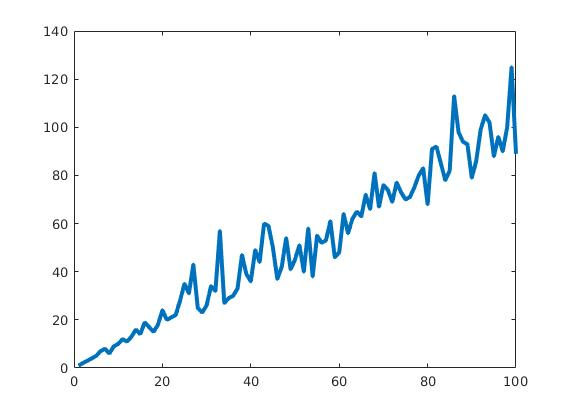
\includegraphics[width=0.8\textwidth]{primo.jpg}
\end{figure}
\begin{figure}[H]
\caption{HPES-0.2 comparato a PageRank}
\centering
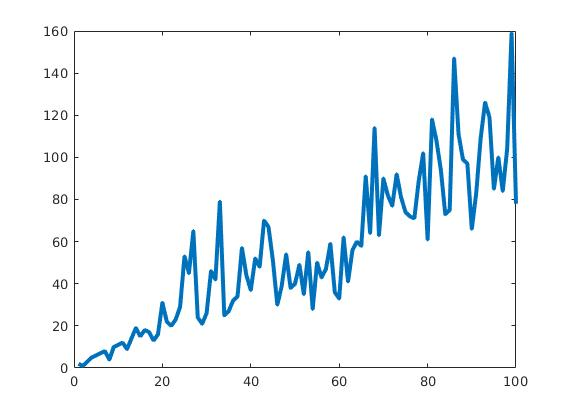
\includegraphics[width=0.8\textwidth]{secondo.jpg}
\end{figure}
\begin{figure}[H]
\caption{HPES-0.3 comparato a PageRank}
\centering
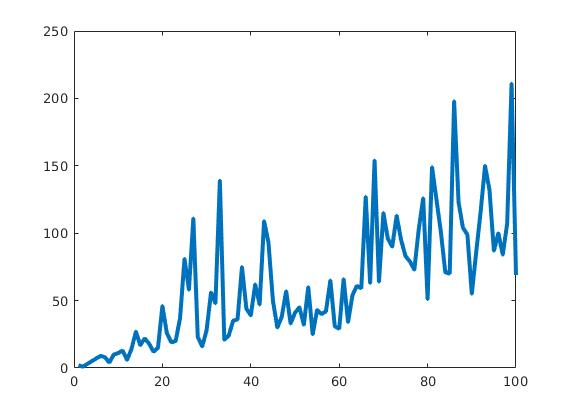
\includegraphics[width=0.8\textwidth]{terzo.jpg}
\end{figure}


\section{Codici} \label{codici}

\begin{lstlisting}[language=Matlab, frame=shadowbox, caption={HPER-$\alpha$}]
function y = HPER_alpha(A, v, tau, itmax, alpha)
unalpha=1-alpha;
n = size(A,1);
v = (1-tau)/sum(v)*v;
e = ones(n,1);
d = A*e;
dang = d==0;
d = d+n*dang;
d = 1./d;
A = A';
beta = 1/sqrt(2*sqrt(n)*(sqrt(n)-1));
w = -ones(n,1)*beta;
w(1) = w(1)+beta*sqrt(n);
Aw = A*(w.*d)+(dang'*(w.*d))*e;
Aw = alpha*w+unalpha*Aw;
wtA = d'.*(w'*A)+sum(w)*(dang'.*d');
wtA = alpha*w'+unalpha*wtA;
A11=alpha+unalpha*(A(1,1)+dang(1))*d(1);
sumA1=alpha+unalpha*sum((A(1,:)+dang').*d');
gamma = A11-(sumA1+1)/sqrt(n)+1;
gamma = n*beta^2*gamma;
s = zeros(n,1);
for i = 1 : n
    s(i) = Aw(i)+wtA(i)-2*gamma*w(i);
    Aii=alpha+unalpha*d(i)*(A(i,i)+dang(i));
    s(i) = Aii-2*w(i)*s(i);
end
s = e-tau*s;
s = 1./s;
y0 = v-2*(w'*v)*w;
y0 = y0.*s;
y0 = y0-2*(w'*y0)*w;
x = rand(n,1);
x = x/sum(x);
dang_red = dang.*d;
for it = 1 : itmax
    Ax = A*(x.*d)+(dang_red'*x)*e;
    Ax = alpha*x+unalpha*Ax;
    y = x-tau*Ax;
    err = norm(v-y);
    y = y-2*(w'*y)*w;
    y = y.*s;
    y = y-2*(w'*y)*w;
    y = y0+x-y;
    if err<1.e-13*norm(y)
        break
    end
    x=y;
end
end
\end{lstlisting}

\begin{lstlisting}[language=Matlab, frame=shadowbox, caption={Metodo di Jacobi}]
function y = Jacobi(A,v,tau,itmax, mod)
n = size(A,1);
e = ones(n,1);
v = (1-tau)/sum(v)*v;
d = A*e;
dang = d==0;
d = d+n*dang;
d = 1./d;
A = spdiags(d,[0],n,n)*A;
A = A';
dang = dang/n;
s = e-tau*(diag(A)+dang);
s = 1./s;
x = rand(n,1);
x = x/sum(x);
for it=1 : itmax
    y = s.*x;
    y = y-tau*(A*y+(dang'*y)*e);
    err = norm(y-v);
    y = v+x-y;
    x=y;
    if err<1.e-13*norm(y)
        break;
    end
    y=s.*y;
end
end
\end{lstlisting}

\begin{lstlisting}[language=Matlab, frame=shadowbox, caption={Metodo delle Potenze}]
function y = Power_method(A, v, tau, itmax, mod)
n = size(A,1);
e = ones(n,1);
d = A*e;
d = d';
dang = d==0;
d = d + dang*n;
dang = dang'/n;
d = 1./d;
x = rand(1,n);
x = x/sum(x);
v = (1-tau)/sum(v)*v;
v=v';
for it=1:itmax
     y = x.*d;
     y = y*A+(x*dang)*e';
     y = tau*y+v;
     err = norm(x-y);
     x = y;
     if err<1.e-13*norm(y)
          break
     end
end
end
\end{lstlisting}




\begin{thebibliography}{99} 

\bibitem{Tudisco} Cipolla Stefano, Di Fiore Carmine, Tudisco Francesco. \textit{Euler-Richardson method preconditioned by weakly stochastic matrix algebras: a potential contribution to Pagerank computation.} Electronic Journal of Linear Algebra, Volume 32, pp. 254-272, 2017.\\
\\

\end{thebibliography}



\end{document}
